This layer involves the various sensors and indicators that interact between the Turing Board and the user directly. This includes a load cell or force-sensing resistor for a weight sensor, a piezoelectric speaker, a printed ArUco symbol, a PWM-capable LED strip, a Tiva C Series Microcontroller, and various electrical components. The weight sensor, speaker, and LEDs communicate directly with the Tiva C Series, while the ArUco symbol is recognized by an Intel RealSense camera which sends the data to the Jetson TX2 via the CV Layer. The Tiva C Series is programmed using C and Assembly via Code Composer Studio 10, while the libraries used for the CV layer mainly use C++ and a generic IDE. This is capable of running on both Windows, MacOS, and Linux.

\subsection{Layer Hardware}
This layer uses a generic piezoelectric speaker (buzzer), a load cell or force-sensing resistor (weight sensor), a printed ArUco symbol generated online (follow anklet), a strip of PWM-capable LEDs approximately 10ft in length, a Tiva C Series, and various electrical components (MOSFETs, resistors, ADC, etc.).

\subsection{Layer Operating System}
This human machine interface layer does not use an operating system. 

\subsection{Layer Software Dependencies}
This layer depends on code done in Code Composer Studio (v10.2) to program the Tiva C Series and drive the various HMI subsystems. We also used the site https://chev.me/arucogen/ to generate our ArUco symbol.

\subsection{Weight Sensor Subsystem}
The weight sensor is currently a safety feature primarily, with future uses in load carrying. When a user is riding on the board, it will detect if they fall off to initiate an emergency stop. When a user attempts to get on the board while in autonomous mode, it will trigger an alert noise to notify the user it is not safe to ride.

\begin{figure}[h!]
	\centering
 	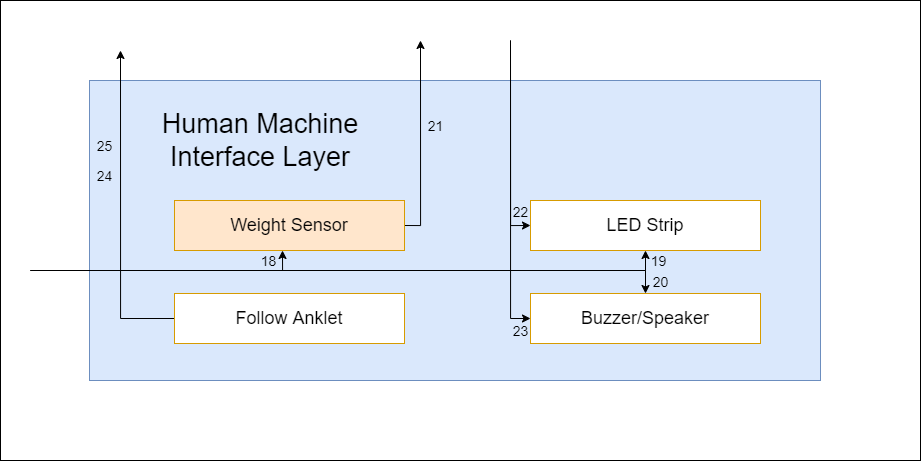
\includegraphics[width=0.60\textwidth]{images/Kendall/Weight Sensor.png}
 \caption{Weight Sensor Subsystem in HMI Layer}
\end{figure}

\subsubsection{Subsystem Hardware}
The weight sensor will implement either a generic load cell or force-sensing resistor in or order to determine the weight/pressure being generated by an item/person placed on top. This detects and senda any weight data to a Tiva C Series to parse and decode.

\subsubsection{Subsystem Operating System}
The weight sensor does not utilize an operating system.

\subsubsection{Subsystem Software Dependencies}
The weight sensor requires the Tiva C Series to read and parse any data. This, in turn, requires Code Composer Studio 10 to create code to parse/read the data and program the Tiva accordingly.

\subsubsection{Subsystem Programming Languages}
Code Composer Studio 10 has code written in C and Assembly.

\subsubsection{Subsystem Data Structures}
The data read in by the sensor is formed into 24-bit "packets" sent along a datastream to the Tiva running at 100kHz. This is done by transmitting one bit per clock using an ADC. This data, which corresponds with an external linear force, is then read and parsed by the Tiva and any relevant data is passed to the other subsystems (LEDs and Buzzer/Speaker) to alert of a weight change.

\subsubsection{Subsystem Data Processing}
The weight sensor does not process any data.

\subsection{Buzzer/Speaker Subsystem}
The buzzer/speaker is used to alert the user if they attempt to step on the board when it is in an autonomous mode. When the weight sensor detects a person attempting to stand on the board when in autonomous mode, the buzzer will begin to sound an alert to notify the user it is unsafe to stand on it.

\begin{figure}[h!]
	\centering
 	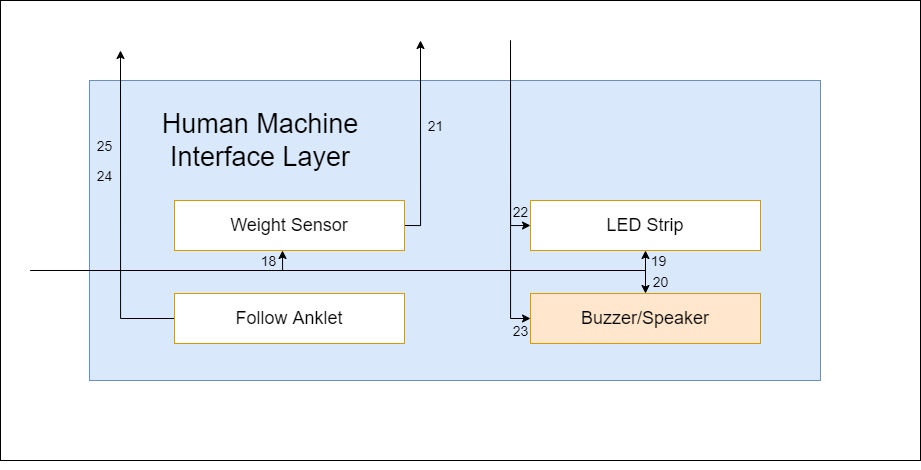
\includegraphics[width=0.60\textwidth]{images/Kendall/Buzzer.png}
 \caption{Buzzer/Speaker Subsystem in HMI Layer}
\end{figure}

\subsubsection{Subsystem Hardware}
This subsystem uses a generic piezoelectric speaker powered and ran by a Tiva C Series microcontroller to emit a sound as an alert on various conditions.

\subsubsection{Subsystem Operating System}
The speaker/buzzer does not use an operating system.

\subsubsection{Subsystem Software Dependencies}
Code Composer Studio 10 is used to program pulse-width modulation (PWM) signals to be sent to the piezoelectric speaker via the Tiva in order to emit a sound of a predetermined frequency and length.

\subsubsection{Subsystem Programming Languages}
Code Composer Studio 10 uses code written in C and Assembly to program the Tiva that communicates with the weight sensor.

\subsubsection{Subsystem Data Structures}
A PWM signal is sent from the Tiva to the speaker using a 32-bit value to determine the frequency at which to emit the sound. The Tiva also uses a 32-bit variable to determine how long to emit the signal for before sending a stop command.

\subsubsection{Subsystem Data Processing}
The speaker/buzzer does not process any data.

\subsection{LED Strip Subsystem}
The LED strip will be used to indicate to the user what mode the Turing Board is currently in. These modes will be differentiated by implementing a different color for each mode. The modes include:
\begin{itemize}
    \item Electric - for electric longboard use
    \item Summoned - for autonomous path finding to the user
    \item Follow-along - for autonomous following of the user wearing the designated
    anklet
\end{itemize}

\begin{figure}[h!]
	\centering
 	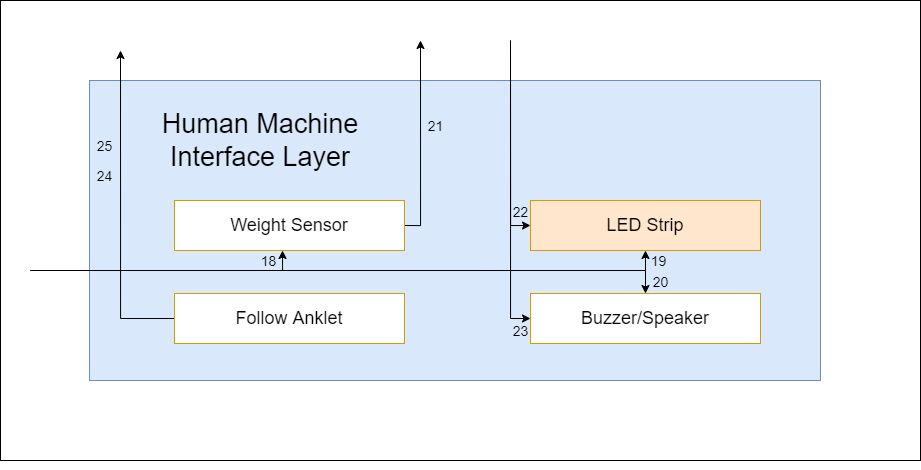
\includegraphics[width=0.60\textwidth]{images/Kendall/LED Strip.png}
 \caption{LED Strip Subsystem in HMI Layer}
\end{figure}

\subsubsection{Subsystem Hardware}
The LEDs are PWM-capable and rated at up to 12V. The Tiva C Series controls the LEDs.

\subsubsection{Subsystem Operating System}
The LEDs do not utilize an operating system.

\subsubsection{Subsystem Software Dependencies}
The LEDs are powered and controlled by the Tiva using Code Composer Studio 10.

\subsubsection{Subsystem Programming Languages}
Code Composer Studio 10 has code written in C and Assembly.

\subsubsection{Subsystem Data Structures}
The LEDs data lines are each fed a 32-bit value, ranging from 0 - 254, corresponding to the Red, Blue, and Green data lines from the Tiva. This, in turn, activates the respective LED color to create various combinations and brightness based on each R/G/B input values.

\subsubsection{Subsystem Data Processing}
The strip has small chips ever few LEDs that passes the 32-bit PWM value to the next chip, allowing the data to be interpreted correctly and for the whole strip to light up at once.

\subsection{Follow Anklet Subsystem}
The Anklet will be a worn feature used for the CV to track and follow the rider in follow-along mode.

\begin{figure}[h!]
	\centering
 	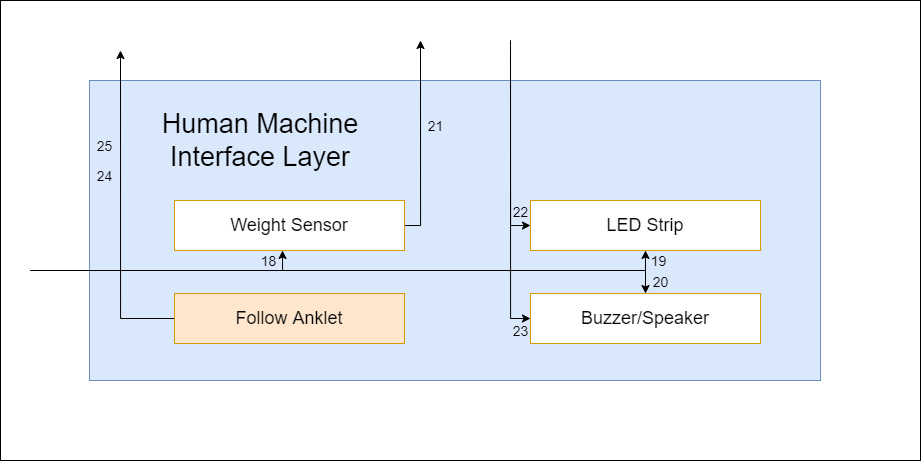
\includegraphics[width=0.60\textwidth]{images/Kendall/Anklet.png}
 \caption{Follow Anklet Subsystem in HMI Layer}
\end{figure}

\subsubsection{Subsystem Hardware}
This subsystem uses an ArUco symbol printed out on a strip of paper long enough to wrap around the user's ankle.

\subsubsection{Subsystem Operating System}
The anklet does not utilize an operating system.

\subsubsection{Subsystem Software Dependencies}
The anklet being detected depends on the ArUco library based on the OpenCV library used to detect and track a generated symbol.

\subsubsection{Subsystem Programming Languages}
The anklet detection software uses C/C++ in the provided libraries required to detect and track the symbol.

\subsubsection{Subsystem Data Structures}
The anklet does not use any data structures.

\subsubsection{Subsystem Data Processing}
The anklet detection software uses an algorithm defined in the ArUco/OpenCV libraries to recognize and track the generated symbol.
